\section{Acoplamiento entre microcintas}%
\label{sec:acoplamiento_entre_microcintas}

Además de simular el acoplamiento entre conductores cilíndricos, se simuló el acoplamiento entre dos microcintas, con una configuración equivalente a la de los conductores cilíndricos. En la figura podemos ver el esquema de la simulación, y en la los resultados. En este caso, en todo el rango de frecuencias las microcintas son eléctricamente largas, por lo que no se cumple la condición cuasi estática para ninguna frecuencia. Es por esto que en los resultados vemos una respuesta similar en forma a la de los conductores para frecuencias altas. El acople en este caso no viene dado por un modelo de parámetros concentrados, sino por uno de líneas de transmisión y radiación.

\begin{figure}[ht]
  \centering
  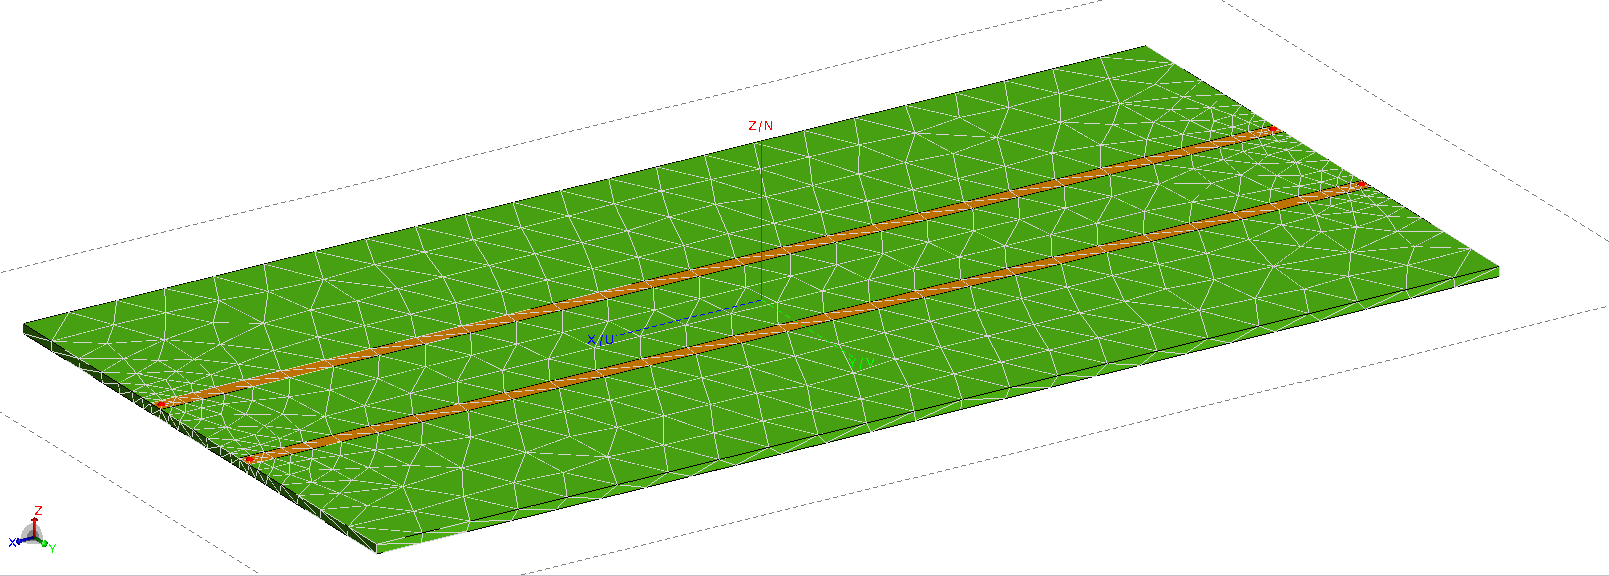
\includegraphics[width=0.6\linewidth]{imagenes/simulacion_microcintas.PNG}
  \caption{Esquema simulado para el acople de microcintas.}%
  \label{fig:imagenes/simulacion_microcintas}
\end{figure}

\begin{figure}[ht]
  \centering
  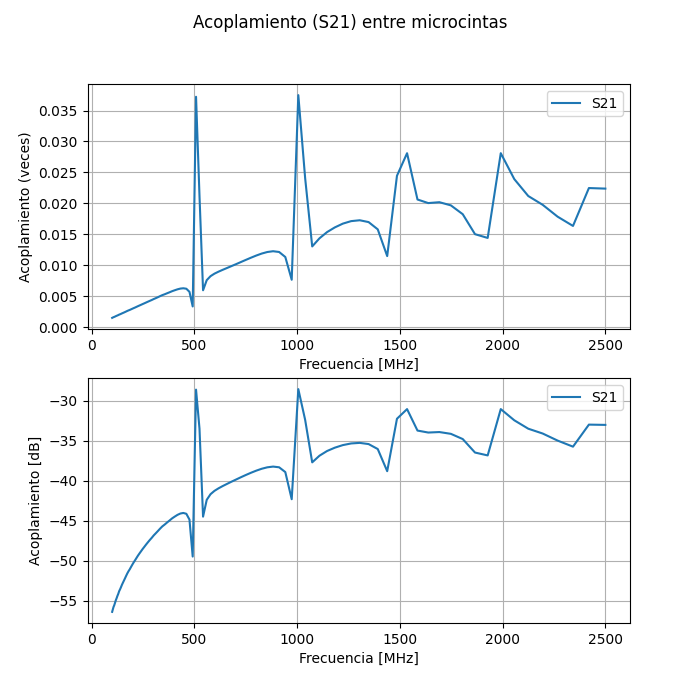
\includegraphics[width=0.6\linewidth]{imagenes/acoplamiento_microcintas_resultado.png}
  \caption{Acople entre las microcintas}%
  \label{fig:imagenes/acoplamiento_microcintas_resultado}
\end{figure}
